\chapter{Elementy kryptografii}

\section{Kryptografia symetryczna oraz asymetryczna}
Współczesną kryptografię można podzielić na kryptografię symetryczną oraz kryptografię asymetryczną. 
W dużym uproszczeniu, w przypadku kryptografii symetrycznej używany jest jeden, wspólny klucz kryptograficzny a w kryptografii asymetrycznej obecna jest para kluczy kryptograficznych - publiczny oraz prywatny. Przez co kryptografia asymetryczna często nazywana jest kryptografią klucza publicznego. 

\subsection{Szyfrowanie symetryczne}
Szyfrowanie symetryczne przy użyciu klucza kryptograficznego ,,miesza'' dane w taki sposób, że nie jest możliwe odzyskanie danych wejściowych bez użycia tego samego klucza. Algorytmy szyfrowania znacznie różnią się między sobą, jednak można pośród nich wyróżnić szyfry blokowe oraz szyfry strumieniowe. \\
Szyfry symetryczne idealnie nadają się do szyfrowania dużych ilości danych. 

\subsection{Szyfrowanie asymetryczne}
Algorytmy używane w szyfrach asymetrycznych opierają się na rozwiązywaniu bardzo trudnych matematycznych problemów. 
Konstrukcja tych szyfrów pozwala niemal natychmiastowo rozwiązać zadany problem (i co za tym idzie odszyfrować dane) mając odpowiedni klucz, a w przypadku nieposiadania owego klucza, problem staje się niemożliwy do rozwiązania w~rozsądnym czasie.
Zwykle wykorzystywane jest tutaj zagadnienie faktoryzacji dużych liczb oraz znajdywania dyskretnych logarytmów. \\
Algorytmy asymetryczne działają na danych o ustalonej długości - zwykle od 1024 do 2048 bitów. Wykorzystywane są one zwykle tylko do przesłania klucza symetrycznego, który jest używane do szyfrowania pozostałej komunikacji. 
Spowodowane jest to tym, że algorytmy symetryczne są dużo bardziej wydajne niż asymetryczne. \\
Szyfrowanie asymetryczne poprawia nieco problem dystrybucji klucza. W odróżnieniu od szyfrowania symetrycznego, wymagane jest użycie $O(N)$ kluczy zamiast $O(N^2)$ \mbox{kluczy}. \\ 
Przykładami algorytmów asymetrycznych jest RSA lub ElGamal. \\ \\ \\
W praktyce rzadko kiedy korzysta się z wyłącznie kryptografii symetrycznej lub wyłącznie asymetrycznej. Zwykle w skład systemów kryptograficznych wchodzą elementy kryptografii symetrycznej jak również asymetrycznej.

\section{Szyfry blokowe}
Jednym z podstawowych elementów systemów kryptograficznych jest szyfr blokowy. Jest to algorytm operujący na bloku danych o ustalonej długości. Długość wynikowego bloku danych jest równa długości bloku podanego na wejściu. \\
Szyfry blokowe oparte są o tzw. ,,sieć substytucji-permutacji''. 
Oznacza to, że dla każdego możliwego bloku jest ustalany dokładnie jeden blok mu odpowiadający. Za pomocą klucza kryptograficznego determinowane jest, który blok odpowiada któremu. \\
Dla zobrazowania tej definicji poniżej znajduje się szyfr o długości bloku równej 4 bity:
\begin{table}[h!]
\centering
\caption{Przykładowy szyfr blokowy o 4-bitowym bloku}
\begin{tabular}{ |c|c| } 
 \hline
	0000: 0010 & 1000: 1111 \\
	0001: 0000 & 1001: 0011 \\
	0010: 0110 & 1010: 1011 \\
	0011: 1101 & 1011: 0001 \\
	0100: 1110 & 1100: 1100 \\
	0101: 0101 & 1101: 1001 \\
	0110: 0100 & 1110: 0111 \\
	0111: 1000 & 1111: 1010 \\
 \hline
\end{tabular}
\end{table} \\
Niezwykle ważną cechą jaka wynika z powyższej charakterystyki szyfru blokowego jest fakt, że znając pewną liczbę par (wiadomość, zaszyfrowana wiadomość), nie ujawnia to żadnych informacji o innych parach, szyfrowanych tym samym kluczem.
Jedyną możliwą formą odszyfrowania wiadomości, nie posiadając klucza, jest wtedy metoda siłowa czyli wypróbowanie wszystkich możliwych kombinacji. 
Biorąc pod uwagę powyższy przykład, mając 16 różnych bloków, liczba ich permutacji wynosi 16! = 20922789888000. 
Prawdziwe szyfry posiadają znacznie większy rozmiar bloku, zwykle od 128 do 256 bitów. Przykładowo dla szyfru z rozmiarem bloku równym 128 bitów, należałoby sprawdzić aż $(2^{128})!$ możliwych kluczy.

\subsection{Tryby pracy szyfrów blokowych}
Nietrudno zauważyć jedną wadę szyfrów blokowych, która znacząco ogranicza proces szyfrowania. 
A mianowicie przy użyciu szyfrów blokowych, jesteśmy w stanie zaszyfrować dane o długości równej długości bloku. 
Zwykle chcielibyśmy jednak szyfrować wiadomości dłuższe niż 16 czy 32 bajty. 
Z tego powodu zostały stworzone uniwersalne konstrukcje, możliwe do użycia z dowolnym szyfrem blokowym, 
pozwalające zaszyfrować dane o dowolnej długości.

\subsubsection{ECB}
Rozwiązaniem przychodzącym natychmiast na myśl jest podzielenie wiadomości na bloki~i zaszyfrowanie każdego bloku oddzielnie. \\
Tryb ten nosi nazwę \textit{ECB (elektroniczna książka kodowa)}. \\
Posiada on niezwykle niebezpieczną wadę. Dany blok wiadomości zostanie zaszyfrowany do zawsze tego samego bloku szyfrogramu. \\
Przykładowo mając wiadomość: $$|\textbf{ABCD}|EFGH|\textbf{ABCD}|IJKL|$$ oraz szyfr blokowy o długości bloku 4 bajty, zaszyfrowana wiadomość będzie wyglądać następująco: $$|\textbf{IEKG}|BKLD|\textbf{IEKG}|FHDL|$$\\
Wadę tę można zobrazować szyfrując w trybie ECB dane dowolnej grafiki. 
Grafika po zaszyfrowaniu nie jest w pełni czytelna ale z pewnością można stwierdzić co na niej jest. \\
Tryb ECB podatny jest również na atak typu \textit{oracle}.

\begin{figure}
    \centering
    \begin{subfigure}{0.3\textwidth}
        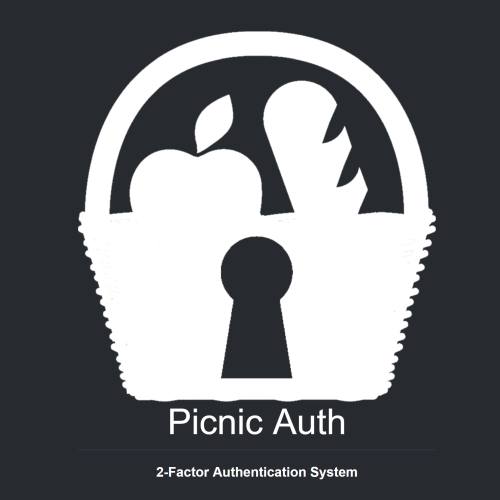
\includegraphics[width=\textwidth]{content/chapters/images/logo}
        \caption{Logo projektu.}
        \label{fig:logo}
    \end{subfigure}
    \begin{subfigure}{0.3\textwidth}
        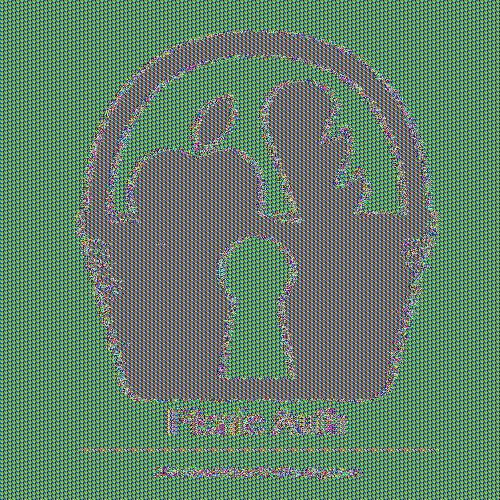
\includegraphics[width=\textwidth]{content/chapters/images/logo-ecb}
        \caption{AES w trybie ECB.}
        \label{fig:logo-ecb}
    \end{subfigure}
    \begin{subfigure}{0.3\textwidth}
        
\includegraphics[width=\textwidth]{content/chapters/images/logo-cbc}
        \caption{AES w trybie CBC.}
        \label{fig:logo-cbc}
    \end{subfigure}
    \caption{Wizualizacja trybów szyfrowania.}
\end{figure}


\subsubsection{ECB}
\subsubsection{CTR}

\subsection{DES}
\subsection{AES}

\section{Szyfry strumieniowe}
Pisząc o szyfrach strumieniowych mam tutaj na myśli natywne szyfry strumieniowe, które zostały stworzone z myślą o pracy w trybie strumieniowym. 
Pomimo istnienia dwóch typów szyfrów strumieniowych - synchroniczny oraz asynchronicznych, w praktyce używany jest prawie wyłącznie pierwszy typ. \\
W odróżnieniu od szyfrów blokowy, które szyfrowały cały blok danych, szyfry strumieniowe szyfrują każdy bit osobno. 
Przy użyciu klucza kryptograficznego generują one wystarczająco długi, pseudolosowy ciąg bitów. 
Następnie wykonywana jest operacja XOR pomiędzy wygenerowanym ciągiem a wiadomością jaką chcemy zaszyfrować. 
Deszyfrowanie polega na ponownym wygenerowaniu ciągu bitów na podstawie klucza a następnie wykonanie operacji XOR na bitach zaszyfrowanej wiadomości oraz tych wygenerowanych z klucza.

\subsection{RC4}
Obecnie najczęściej spotykanym szyfrem strumieniowym jest RC4. Mimo, że wielokrotnie wykazano wiele podatności w konstrukcji RC4, szyfr ten jest ciągle używany w protokołach takich jak TLS czy WEP. \\
Schemat działania algorytmu jest niezwykle prosty. 
Składa się z inicjalizacji klucza oraz generacji pseudolosowego ciągu. \\
W etapie inicjalizacji klucza tworzona jest tablica permutacji S, składają się z 256 bajtów. 
Początkowo znajdują się w niej kolejne liczby od 0 do 255. 
Następnie dokonywane jest przejście po elementach tablicy, korzystając z indeksu \textit{i}. Na każdym kroku pętli obliczany jest indeks \textit{j}, poprzez dodanie aktualnej wartości \textit{j} (zaczynającej się od 0) do wartości klucza znajdującej się pod indeksem \textit{i} oraz do wartości tablicy S znajdującej się pod indeksem \textit{i}. W przypadku, gdyby któryś z indeksu wyszedł poza zakres rozpatrywanych tablic, używa się operacji modulo długość tablicy. Mając obliczony indeks \textit{j} zamienia się element $S[i]$ z elementem $S[j]$. \\
Do wygenerowania pseudolosowego ciągu wykorzystywana jest wcześniej stworzona tablica permutacji S. W pierwszej kolejności dla każdego indeksu \textit{i}, obliczany jest indeks $j := j + S[i]$. 
Następnie zamienione są wartości $S[i]$ oraz $S[j]$. W celu otrzymania bajtu, który zostanie wykorzystany do zaszyfrowania wiadomości, pobierana jest wartość $S[S[i] + S[j]]$ z tablicy~S.

\subsection{Salsa20}
W porównaniu do RC4, Salsa20 jest relatywnie nowym szyfrem strumieniowym, stworzonym przez Daniela J. Bernsteina. 
Bazuje on na operacjach \textit{ARX (add–rotate–xor)}, to jest operacji składających się z dodawania modulo, obrotów bitowych oraz funkcji \textit{XOR}. 
Zaletą stosowania szyfrów \textit{ARX} jest to, że odporne są one na ataki czasowe, polegające na mierzeniu czasu,
jaki potrzebny jest do przeprowadzenia operacji kryptograficznych. \\
Niezwykle interesującą cechą szyfru Salsa20 jest możliwość rozpoczęcia procesu odszyfrowywania od dowolnego miejsca w strumieniu danych. Mając więc duży plik, możliwe jest odszyfrowywanie tylko tej jego części, która nas interesuje. \\
Na chwilę obecną nie są znane żadne praktyczne ataki na szyfr Salsa20, może on zostać użyty jako alternatywa do szyfru blokowego AES.

\section{Kryptograficzna funkcja skrótu}
Funkcją skrótu nazywana jest funkcja, która dla danych wejściowych o dowolnym rozmiarze zwraca dane o z góry ustalonej długości. Funkcje skrótu znajdują zastosowanie w takich dziedzinach jak struktury danych (tablice mieszające, filtr Blooma), algorytmy dopasowania wzorca (algorytm Karpa-Rabina) czy też w kryptografii. \\ \\
Aby funkcja skrótu mogła zostać użyta w systemach kryptograficznych musi posiadać ona szereg parametrów. \\
Jednym z nich jest odporność na kolizje. Kolizją nazywamy przypadek, gdy dla dwóch różnych argumentów funkcja skrótu zwraca ten sam wynik. Nie jest oczywiście możliwe, aby całkowicie uniknąć kolizji, gdyż zbiór danych o dowolnym rozmiarze jest mapowany na zbiór skończony, zależy nam jednak aby proces znajdywania kolizji dla określonych danych był uważany za ,,trudny''. (Przez ,,trudny'' należy tutaj rozumieć problem, który nie jest możliwy do rozwiązania w rozsądnej ilości czasu.) \\
Kolejny z parametrów jest częściowo związany z poprzednim. Zależy nam, aby rozpatrywana funkcja była funkcją jednokierunkową. Oznacza to, że dla danego wyniku funkcji skrótu, znalezienie argumentu jest również problemem ,,trudnym''.
(Sam fakt istnienia funkcji jednokierunkowych nie został formalnie udowodniony. \cite{oneway}) \\
Niezwykle ważne jest też, aby nawet niewielka zmiana danych wejściowych, spowodowała znaczną zmianę danych otrzymanych na wyjściu (wymagane jest aby przynajmniej połowa bitów uległa zmianie).

\subsection{Message Digest 5}
Funkcja MD5 jest wykorzystywana do generowania 128-bitowego skrótu. Została stworzona przez Rona Rivesta w 1991 roku. \\
W uproszczeniu, algorytm MD5 można przedstawić w następujących krokach \cite{crypto101}:
\begin{enumerate}
	\item Dodanie dopełnienia. W pierwszej kolejności dopisywany jest jeden bit o wartości 1, a następnie dopisywane są zera, aż do momentu, gdy długość danych wynosić będzie 448 bitów modulo 512. Dopełnienie dopisywane jest nawet w przypadku, gdy długość danych wynosi 448 bitów.
	\item Pozostałe 64 bity wypełniane są liczbą reprezentującą długość wiadomości (sprzed wypełnienia) modulo $2^{64}$. 
	\item Inicjalizacja stanu MD5 w postaci czterech 32-bitowych zmiennych A, B, C i D. Są one inicjalizowane stałymi zdefiniowanymi w specyfikacji (przedstawione w systemie szesnastkowym): 
		\begin{itemize}
			\item A: 01 23 45 67
			\item B: 89 ab cd ef
			\item C: fe dc ba 98
			\item D: 76 54 32 10
		\end{itemize}
	\item Dane wejściowe dzielone są na bloki po 512 bitów. Kolejno na każdym z bloków wykonywane są operacje bitowe zmieniające zmiennych. 
	\item Wynikiem działania algorytmu jest 128-bitowa wartość składająca się z omawianych czterech zmiennych w kolejności A, B, C, D.
\end{enumerate} 
Szczegółowa specyfikacja algorytmy znajduje się w dokumencie RFC 1321 \cite{md5rfc}. \\
Analiza kryptograficzna funkcji MD5 wykazała wiele podatności i błędów przez co obecnie nie jest wskazane używanie MD5 w zastosowaniach kryptograficznych. 
W roku 2004 została opublikowana praca wykazująca podatność funkcji MD5 na ataki kolizyjne (ang. collision attack) \cite{md5cert}. Cztery lata później został znaleziony atak na kody uwierzytelnienia wiadomości bazujące na funkcji MD5 \cite{md5hmac}.

\subsection{Secure Hash Algorithm 1}
SHA-1 jest funkcją bazującą na MD4 (podobnie jak MD5), o długości skrótu wynoszącej 160 bitów \cite{cryptoirf}. \\
Wewnętrzny stan funkcji składa się z pięciu zmiennych: A, B, C, D oraz E, każda o rozmiarze 32 bitów. \\
Pseudokod algorytmu można przedstawić w następujących krokach:
\begin{enumerate}
	\item Inicjalizacja zmiennych następującymi stałymi (przedstawione w systemie szesnastkowym):
		\begin{itemize}
			\item A = 0x67452301
			\item B = 0xEFCDAB89
			\item C = 0x98BADCFE
			\item D = 0x10325476
			\item E = 0xC3D2E1F0
		\end{itemize}
	\item Zaaplikowanie dopełnienia:
		\begin{enumerate}
			\item Dopisanie na koniec danych bitu o wartości 1. \\ 
			Przykładowo jeśli przetwarzane są dane \textit{01011001}, to są one dopełniane do \textit{010110011}.
			\item Następnie dopisywane są bity o wartości 0, aż do momentu, gdy długość danych wynosić będzie 448 bitów modulo 512. \\
			Mając dane \textit{00101101 01000010 10011101 10001010 00101101 10011101}, po zastosowaniu dopełnienia z kroku (a) otrzymujemy \textit{00101101 01000010 10011101 10001010 00101101 10011101 1}. Jako że długość danych wynosi 49 bitów, wymagane jest dopisanie 399 zer. Po zastosowaniu dopełnienia otrzymujemy (reprezentacja heksadecymalna): \\
			\textit{2d429d8a 2d9d8000 00000000 00000000 \\ 
					00000000 00000000 00000000 00000000 \\ 
					00000000 00000000 00000000 00000000 \\ 
					00000000 00000000 }
			\item W ostatnim kroku na miejsce ostatnich 64 bitów dopisywana jest długość danych. 
			\textit{2d429d8a 2d9d8000 00000000 00000000 \\ 
					00000000 00000000 00000000 00000000 \\ 
					00000000 00000000 00000000 00000000 \\ 
					00000000 00000000 00000000 00000031 }
		\end{enumerate}
	\item Podzielenie wiadomości na 512-bitowe bloki.
	\item Dla każdego z bloków należy wykonać następujące operacje:
		\begin{enumerate}
			\item Podzielenie bloku na szesnaście 32-bitowych części $w[i], 0 \leq i \leq 15$.
			\item Rozszerzenie 16 części do 80 korzystając ze wzoru: \\
				$w[i] = (w[i-3] \xor w[i-8] \xor w[i-14] \xor w[i-16]) << 1$
			\item Inicjalizacja zmiennych pomocniczych dla danego bloku
				\begin{itemize}
					\item a = A
					\item b = B
					\item c = C
					\item d = D
					\item e = E
				\end{itemize}
			\item Dla każdej z 80 części $w[i]$ należy wykonać:
				\begin{enumerate}
					\item jeżeli $0 \leq i \leq 19$ 
				        \begin{itemize} 
				        	\item $f = (b \BitAnd c) \BitOr ((\BitNeg b) \BitAnd d)$
				            \item $k = 0x5A827999$
				        \end{itemize}
					\item jeżeli $20 \leq i \leq 39$
						\begin{itemize} 
            				\item $f = b \xor c \xor d$
            				\item $k = 0x6ED9EBA1$
            			\end{itemize}
				    \item jeżeli $40 \leq i \leq 59$
				        \begin{itemize} 
				        	\item $f = (b \BitAnd c) \BitOr (b \BitAnd d) \BitOr (c \BitAnd d)$ 
            				\item $k = 0x8F1BBCDC$
			            \end{itemize}
        			\item jeżeli $60 \leq i \leq 79$
        				\begin{itemize} 
				            \item $f = b \xor c \xor d$
    	        			\item $k = 0xCA62C1D6$
            			\end{itemize}
            		\item następnie
            			\begin{itemize}
            				\item $t = (a <<< 5) + f + e + k + w[i]$ 
					        \item $e = d$ 
					        \item $d = c$
					        \item $c = b <<< 30$
					        \item $b = a$ 
					        \item $a = t$ 
            			\end{itemize}
				\end{enumerate}
			\item Aktualizacja wewnętrznego stanu funkcji			
				\begin{itemize}
					\item A = A + a
					\item B = B + b
					\item C = C + c
					\item D = D + d
					\item E = E + e
				\end{itemize}
		\end{enumerate}
	\item Zwrócenie wyniku w postaci: \\
		$(A << 128) \BitOr (B << 96) \BitOr (C << 64) \BitOr (D << 32) \BitOr E$
\end{enumerate}
W dokumencie RFC 3174 zostały zawarte szczegóły dotyczące algorytmu, jak również przykładowa implementacja \cite{sha1rfc}. \\ \\
Podobnie jak MD5, funkcja SHA-1 również nie jest uważana za bezpieczną. \\
Do roku 2017 wszystkie przedstawione ataki uznawane były za niepraktyczne z uwagi na zbyt dużą moc obliczeniową, jaka byłaby potrzebna do ich wykonania.
Przykładem może być tutaj atak opublikowany w październiku 2015 roku o nazwie \textit{The SHAppening}. Koszt wynajęcia sprzętu potrzebnego do przeprowadzenia ataku (wygenerowania jednej kolizji) estymowany był na 75 000 - 120 000 dolarów amerykańskich \cite{shap}. \\
Pierwszy praktyczny atak na SHA-1 został ogłoszony w lutym 2017 roku. Zostały wygenerowane dwa pliki w formacie PDF, dla których wynik funkcji skrótu SHA-1 jest taki sam. Wszystkie systemy, w których wykorzystywana jest funkcja SHA-1 są narażone na ten atak, przykładowo umożliwia on fałszowanie podpisów cyfrowych dokumentów, czy też certyfikatów HTTPS. \cite{shatt}

\subsection{Secure Hash Algorithm 2}
SHA-2 jest rodziną funkcji składającą się z \mbox{SHA-224}, \mbox{SHA-256}, \mbox{SHA-384}, \mbox{SHA-512}, \mbox{SHA-512/224}, \mbox{SHA-512/256}. Funkcje te generują skróty o długościach odpowiednio: 224, 256, 384, 512, 224 oraz 256 bitów.

\subsubsection{SHA-256}
Jedną z najczęściej używanych funkcji z rodziny SHA-2 jest SHA-256. Proces uzyskiwania skrótu SHA-256 jest następujący:
\begin{enumerate}
	\item Inicjalizacja stanu wewnętrznego funkcji (przedstawione w systemie szesnastkowym):
		\begin{itemize}
			\item A = 0x6a09e667
			\item B = 0xbb67ae85
			\item C = 0x3c6ef372
			\item D = 0xa54ff53a
			\item E = 0x510e527f
			\item F = 0x9b05688c
			\item G = 0x1f83d9ab
			\item H = 0x5be0cd19
		\end{itemize}
	\item Inicjalizacja pomocniczych stałych. \\
			$$
			k[0..63] := \\
			\begin{matrix}
				0x428a2f98, & 0x71374491, & 0xb5c0fbcf, & 0xe9b5dba5, \\
				0x3956c25b, & 0x59f111f1, & 0x923f82a4, & 0xab1c5ed5, \\
				0xd807aa98, & 0x12835b01, & 0x243185be, & 0x550c7dc3, \\
				0x72be5d74, & 0x80deb1fe, & 0x9bdc06a7, & 0xc19bf174, \\
				0xe49b69c1, & 0xefbe4786, & 0x0fc19dc6, & 0x240ca1cc, \\
				0x2de92c6f, & 0x4a7484aa, & 0x5cb0a9dc, & 0x76f988da, \\
				0x983e5152, & 0xa831c66d, & 0xb00327c8, & 0xbf597fc7, \\
				0xc6e00bf3, & 0xd5a79147, & 0x06ca6351, & 0x14292967, \\
				0x27b70a85, & 0x2e1b2138, & 0x4d2c6dfc, & 0x53380d13, \\
				0x650a7354, & 0x766a0abb, & 0x81c2c92e, & 0x92722c85, \\
				0xa2bfe8a1, & 0xa81a664b, & 0xc24b8b70, & 0xc76c51a3, \\
				0xd192e819, & 0xd6990624, & 0xf40e3585, & 0x106aa070, \\
				0x19a4c116, & 0x1e376c08, & 0x2748774c, & 0x34b0bcb5, \\
				0x391c0cb3, & 0x4ed8aa4a, & 0x5b9cca4f, & 0x682e6ff3, \\
				0x748f82ee, & 0x78a5636f, & 0x84c87814, & 0x8cc70208, \\
				0x90befffa, & 0xa4506ceb, & 0xbef9a3f7, & 0xc67178f2  	
			\end{matrix}
			$$
	\item Zaaplikowanie dopełnienia. Proces ten przebiega identycznie jak w przypadku SHA-1.
	\item Podzielenie wiadomości na 512-bitowe bloki.
	\item Dla każdego z bloków należy wykonać następujące operacje:
		\begin{enumerate}
			\item Podzielenie bloku na szesnaście 32-bitowych części $w[i], 0 \leq i \leq 15$.
			\item Rozszerzenie 16 części do 64 korzystając ze wzoru: \\
				$s0 := (w[i-15] >>> 7) \xor (w[i-15] >>> 18) \xor (w[i-15] >> 3)$ \\
			    $s1 := (w[i-2] >>> 17) \xor (w[i-2] >>> 19) \xor (w[i-2] >> 10)$ \\
				$w[i] := w[i-16] + s0 + w[i-7] + s1$
			\item Inicjalizacja zmiennych pomocniczych dla danego bloku
				\begin{itemize}
					\item a = A
					\item b = B
					\item c = C
					\item d = D
					\item e = E
					\item f = F
					\item g = G
					\item h = H
				\end{itemize}
			\item Dla każdej z 64 części $w[i]$ należy wykonać:
				\begin{itemize}
					\item $S1 := (e >>> 6) \xor (e >>> 11) \xor (e >>> 25)$
			        \item $ch := (e \BitAnd f) \xor ((\BitNeg e) \BitAnd g)$
			        \item $t1 := h + S1 + ch + k[i] + w[i]$
			        \item $S0 := (a >>> 2) \xor (a >>> 13) \xor (a >>> 22)$
			        \item $m := (a \BitAnd b) \xor (a \BitAnd c) \xor (b \BitAnd c)$
			        \item $t2 := S0 + m$
			        \item $h := g$
			        \item $g := f$
			        \item $f := e$
			        \item $e := d + t1$
			        \item $d := c$
			        \item $c := b$
			        \item $b := a$
			        \item $a := t1 + t2$
				\end{itemize}
			\item Aktualizacja wewnętrznego stanu funkcji			
				\begin{itemize}
					\item A = A + a
					\item B = B + b
					\item C = C + c
					\item D = D + d
					\item E = E + e
					\item F = F + f
					\item G = G + g
					\item H = H + h
				\end{itemize}
		\end{enumerate}
	\item Zwrócenie wyniku w postaci: \\
		$(A << 224) \BitOr (B << 192) \BitOr (C << 160) \BitOr \\ 
		 (D << 128) \BitOr (E << 96) \BitOr (F << 64) \BitOr (G << 32) \BitOr H$
\end{enumerate}
W porównaniu do SHA-1 są znacznie odporniejsze na kolizję, dzięki czemu zalecane jest ich używanie w zastosowaniach takich jak podpisy cyfrowe czy uwierzytelnianie wiadomości.

\subsection{Secure Hash Algorithm 3}
Wewnętrzna budowa funkcji z rodziny SHA-3 znacząco się różni w odniesieniu do omawianych wcześniej. 
Poprzednie funkcje oparte były o schemat Merkle–Damgård. Funkcje z rodziny SHA-3 oparte są o tak zwaną ,,architekturę gąbki''. W obu przypadkach funkcja zawiera wewnętrzny stan. Różnica jest jednak w sposobie otrzymywania wyniku na podstawie tego stanu. Poprzednio zwrócenie przez funkcję wyniku było równoznaczne ze zwróceniem wewnętrznego stanu funkcji. W przypadku SHA-3 tak się nie dzieje. Wewnętrzny stan przepuszczany jest kolejne cykle algorytmu. Na wynik funkcji składają się części wewnętrznego stanu, pobierane w kolejnych cyklach. Skutkuje to tym, że nigdy nie jest ujawniany cały wewnętrzny stan funkcji. \\
Ulepszona wewnętrzna konstrukcja algorytmu zapobiega atakom typu ,,length extension'', na który podatne są funkcje MD5, SHA-1 oraz SHA-2 \cite{keccak}.

\section{Kod uwierzytelnienia wiadomości}

\section{MAC bazujący na funkcji skrótu}

\section{Pojęcia entropii}
